%\documentclass[fleqn]{book}
\documentclass[11pt]{amsbook}

\usepackage[turkish]{babel}

%\usepackage{../HBSuerDemir}	% ------------------------
\usepackage{../Ceyhun}	% ------------------------
\usepackage{../amsTurkish}

\begin{document}
% ++++++++++++++++++++++++++++++++++++++
\hPage{110}
% ++++++++++++++++++++++++++++++++++++++

%\begin{tanit}
$Ç_0$ içinde iki Euler çizgesidir. $$ (Y_1 \cup a_0) \bigoplus ( Y_2 \cup a_0) = Y_1 \bigoplus Y_2$$
ise hem $Ç_0$ hem de Ç içinde bir Euler çizgesidir. \\
%\end{tanit}
%When I try to use \begin{tanit}, it gives an error. And I am also not sure about using it because this "tanım" is not starting in my page.
%That's why I commented it out.

Teorem 3.1.3 ün bir genellemesi olarak, $d_i$ ve $d_j$ düğümleri arasında $2n$ sayıdaki yolların da $\bigoplus$ altında bir Euler çizgesi oluşturacağını gösterebiliriz. Bu özellikleri \reffig{fig:3.1.1} de gösterilen çizge üzerinde açıklayalım.
$$E_1 = (a_1,a_4,a_5)$$
$$E_2 = (a_2,a_5,a_6)$$
$$E_3 = (a_3,a_4,a_6)$$ $Ç(4,6)$ çizgesindeki üç ayrı Euler çizgesidir.

\begin{figure}[htb]
	\centering
	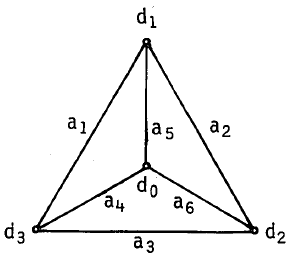
\includegraphics[width=0.45\textwidth]{images/ceyhun-110-fig01}
	\caption{E ve Y altçizgelerinin $\bigoplus$ altındaki özelliklerinin açıklanması.}
	\label{fig:3.1.1}
\end{figure}

\end{document}